\documentclass[12pt,a4paper,twoside,english,fleqn]{article}

\setlength{\parskip}{\medskipamount}
\setlength{\parindent}{0pt}
\usepackage{amsmath}
\usepackage{graphicx}
\usepackage{listings}
\usepackage[xcolor,framemethod=tikz,nobreak]{mdframed}
\usepackage{units}

%\textwidth18cm
\textwidth16cm
%\hoffset-1.5cm

\textheight24cm
\voffset-1.5cm

\setlength{\oddsidemargin}{0.3cm}
\setlength{\evensidemargin}{0.3cm}


\begin{document}

% set code environment (lstlisting)
\lstset{language=bash}
\lstset{basicstyle=\ttfamily}
\lstset{columns=fullflexible}

\mdfsetup{
  font={\footnotesize\sffamily},
  frametitlefont={\large\sffamily\bfseries},
  middlelinecolor=red,
  middlelinewidth=2pt,
  backgroundcolor=red!10,
  roundcorner=10pt,
  innerbottommargin=20pt,
  innerleftmargin=20pt,
  innerrightmargin=20pt,
  frametitleaboveskip=20pt}

\title{\vspace{-3cm}The \emph{clustering} Tutorial\\
                    -- version 0.12 --}
\author{Florian Sittel\\
        Biomolecular Dynamics / Institute of Physics / University of Freiburg}
\maketitle

\section{Introduction}
The shell commands invoking the \emph{clustering} program are written in
multiple lines to emphasize the single parameters and options given to the
program. This is, however, only for better readibility in this tutorial.
All commands should be executed in a single line, without the additional line
breaks.


\section{Preparing the data}
Apply a suitable dimension reduction method (e.g. PCA) on the data and select a
limited number of essential coordinates.
It is important not to exceed the maximum dimensionality for the given sampling
when using a density-based clustering approach.
Too high dimensionality will suffer from the 'Curse of Dimensionaliy'.
A good estimate, e.g. for a ten dimensional data set is a sampling of $> 10^6$
frames.

The input data for the \emph{clustering} package needs to be column-oriented,
space-separated plain text.

From now on, let's assume we have prepared input data for \emph{clustering} in
the file {\ttfamily coords}.

\begin{mdframed}[frametitle={Test data available!}]
  If you want to get your hands dirty right away and do not yet have suitable
  data, you can get a data set at
  http://www.moldyn.uni-freiburg.de/software/aib9.pca.reduced.bz2.

  Download the data, e.g., with {\ttfamily wget}, unpack it with
  {\ttfamily bzip2} and create a symlink called 'coords' to be in line with
  the rest of the tutorial:
  \begin{lstlisting}
  wget http://www.moldyn.uni-freiburg.de/software/aib9.pca.reduced.bz2

  bunzip2 aib9.pca.reduced.bz2

  ln -s aib9.pca.reduced coords
  \end{lstlisting}

  If your computer is missing any of these programs, install them (or let the
  sysadmin do it). If they are not available, get a decent Linux distribution...

  The data consists of $\sim 1.4 \cdot 10^6$ frames of a simulation of the
  peptide Aib9 (for more information on this data set, see \cite{Buchenberg15}),
  reduced to four essential coordinates based on a principal
  component analysis using dihedral angles.
  Fig. \ref{fig:pca_proj} shows the 2D projections along principal components
  1 \& 2 and 3 \& 4 to give an impression of the free energy landscape.
\end{mdframed}

\begin{figure}
  \centerline{
    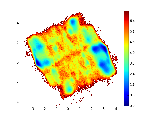
\includegraphics[width=7cm] {aib9_pca_pc1_pc2}
    \hspace{1cm}
    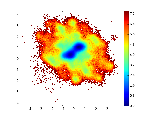
\includegraphics[width=7cm] {aib9_pca_pc3_pc4}}
  \caption{\label{fig:pca_proj}
    Projections of (left) first and second principal components
    and (right) third and fourth principal components of
    Aib9 based on PCA of dihedral angles.}
\end{figure}



\section{The optimal radius for density clustering}
The density-based clustering algorithm depends heavily on the radius, which
distinguishes neighboring frames from non-neighboring frames.
The radius, however, is given as an input parameter to the clustering and has
to be provided by the user.

Yet, there is a simple but effective method to identify the optimal radius for
the clustering run itself. Since microstates in a microcanonical ensemble
statistically show the behavior of a Boltzmann distribution, their population
(ordered in descending order) should decay exponentially.
As we treat every single frame as a microstate (by assigning a neighborhood
and estimating a local free energy / population), we can directly use this
feature.

Run the command

\begin{lstlisting}
  clustering density -f coords
                       -R 0.1 0.2 0.3 0.4 0.5 0.6 0.7 0.8
                       -p pop
                       -d fe
                       -n 12
                       -v
\end{lstlisting}

to compute the free energies and populations for a set of different radii.
The single parameters are
\begin{itemize}
  \item -f: The input coordinates
  \item -R: A list of radii (in units of the input coordinates)
  \item -p: Filename prefix for the output files of populations.
            For every radius, a file 'PREFIX\_RADIUS' will be written
            to disk, e.g. 'pop\_0.2'.
  \item -d: The same as '-p', but for free energies.
  \item -n: The number of parallel threads to use (for SMP machines).
  \item -v: Verbose mode with lots of output.
\end{itemize}

Using a shell like bash, you can generate a list of radii on the fly via the
{\ttfamily seq} command, without having to write them out manually:
\begin{lstlisting}
  clustering density -f coords -R $(seq 0.1 0.1 0.8) ...
\end{lstlisting}

For every radius, sort the frame populations in descending order and fit to an
exponential decay (or visually inspect instead of fitting).
The optimal radius is the one that fits best.

Let's assume from now on that 0.3 is the radius of our choice for the given
data set.

\begin{mdframed}[innertopmargin=20pt]
  Running above command for the Aib9 data set took about 20 minutes on
  12 hyperthreaded cores of a Core i7-4930K.
  Figure \ref{fig:pops_ordered} shows the resulting populations for various
  radii, reordered from highest to lowest population.
  From this plot, we select 0.3 as optimal radius, since it is, on the one
  hand, small enough to resolve local densities and, on the other hand, shows
  near-exponential decay. Pro-tip: use log-plots...
\end{mdframed}


\begin{figure}
  \centerline{
    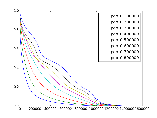
\includegraphics[width=10cm] {pops_ordered}}
  \caption{\label{fig:pops_ordered}
      Populations of Aib9 frames for different hypersphere radii,
      ordered from highest populated to lowest populated frame.
      Populations have been normalized to max(pop) = 1.}
\end{figure}



\section{Geometric clustering via density screening}
Computation of the per-frame free energies and local neighborhoods is very
demanding. Therefore, we will store the intermediate results in files and reuse
them when needed.

\subsection{Computing the local neighborhood for a given radius}
The free energies have already been computed (and hopefully stored by defining
'-d'!) in the radius evaluation step.
Here, we will compute the local neighborhoods per frame, reusing the previously
computed free energies:
\begin{lstlisting}
  ln -s fe_0.300000 fe

  clustering density -f coords
                       -r 0.3
                       -D fe
                       -b nn
                       -n 12
                       -v
\end{lstlisting}
The (new) options are
\begin{itemize}
  \item -r: Use radius of 0.3 for all computations.
  \item -D: Reuse free energies (radius 0.3), that already have been
            computed in the previous step (symlinked to 'fe')
  \item -b: Compute neighborhood (i.e. nearest neighbors) for the given
            radius and store for later reuse in file 'nn'.
\end{itemize}


\begin{mdframed}[innertopmargin=20pt]
  Running above command for the Aib9 data set took about 30 minutes on
  12 hyperthreaded cores of a Core i7-4930K.
\end{mdframed}




\subsection{Screening the FEL\label{sec:screening}}
Given the readily computed free energies (fe) and neighborhoods (nn)
per frame for the selected radius,
we continue the clustering by screening the free energy landscape.
This means, we choose a (initially low) free energy cutoff, select all frames
below and combine them into microstates, if their respective distance is closer
then a certain threshold, which is automatically computed for the given data
set.

This is done repeatedly, with increasing free energy cutoffs.
The end result will be multiple plain-text files, one for each cutoff, that
define cluster trajectories. Their format is a single column of integers, which
act as a membership id of the given frame (identified by the row number) to
a certain microstate.
For each file, the microstate ids start with the value 1 and are numbered
incrementally. All frames above the given free energy threshold are assigned to
state 0, which acts as a kind of melting pot for frames with unknown
affiliation.

To screen the free energy landscape, run the command
\begin{lstlisting}
  clustering density -f coords
                       -r 0.3
                       -D fe
                       -B nn
                       -T 0.1 0.2
                       -o clust
                       -n 12
                       -v
\end{lstlisting}
The options are
\begin{itemize}
  \item -B: Reuse neighborhood information stored in nn.
  \item -T: Run the free energy screening, beginning at a threshold of 0.1 kT
            and increasing per step by 0.2 kT until the maximum free energy
            of this data set is reached.
            Additionally, you can define the maximum free energy for the
            screening, e.g. '-T 0.1 0.2 10.0' to go to 10 kT.
            Alternatively, define '-T -1' for a default setting, starting at
            0.1, stepping by 0.1 and going up to the maximum free energy.
  \item -o: Define a basename for the resulting cluster files. The current free
            energy cutoff will be appended as a suffix, e.g. 'clust\_0.10',
            'clust\_11.30', etc. \textbf{Warning: If you do not specify a name
            for the output files, nothing will be written to disk! The only
            result you will get is a heated computer and a waste of time.}
\end{itemize}

Do not worry if there are still frames denoted by 0 in the cluster file of
highest free energy. The \emph{clustering} program rounds the maximum free
energy to 2 decimal places for screening, which may result in a cutoff that is
slightly lower the true maximum. Thus there may be frames left, which are not
assigned to a microstate since they are not below the cutoff.

However, since we are going to generate microstates from selecting the basins
of the microstates and 'filling up' the free energy landscape from bottom to
top, these states are not interesting on their own, anyhow, and will be
assigned to a distinct microstate in the next step.

\begin{mdframed}[innertopmargin=20pt]
  Running above command for the Aib9 data set took about 1.75 hours on
  12 hyperthreaded cores of a Core i7-4930K.
\end{mdframed}



\section{Generating microstates}
\subsection{The network of geometrically clustered states
            \label{sec:network_generation}}
The net result of the screening process (section \ref{sec:screening}) is a list
of files (here: clust\_*) defining the cluster membership per frame for
different free energy cutoffs. Using these memberships, we can derive a network
of microstates that reflects their respective geometrical similarity.
The network has a (multi-)tree structure, with nodes defining separate
microstates at the various free energy levels. In case two (or more) clusters
grow big enough to be geometrically close, they will be merged into a single
node at the free energy level, at which they are not distinguishable from a
single state.

If the metastable states of the free energy landscape are geometrically diverse
enough, the network will form several trees in parallel, without them being
joined at the highest free energy level. Of course, you can add a virtual root
node at a free energy level above the maximum to join all trees into a single
tree, however this has to be done manually.
The \emph{clustering} program will not artificially join the separate trees.

To create a network from the screening data, run
\begin{lstlisting}
  clustering network -p 500
                       --step 0.2
                       -v
\end{lstlisting}
The input parameters stand for
\begin{itemize}
  \item -p: Filter out all nodes (i.e. microstates) with populations less then
            a given number. This parameter is very helpful to control the
            resolution of the resulting model (i.e. network). Artificially
            small microstates (e.g. single frames with highly distorted
            geometry, which actually do not form a metastable state) can be
            omitted by this option.
  \item --step: Set stepping for network generation, i.e., free energy
                difference between nodes.
\end{itemize}

This command will generate several files:
\begin{itemize}
  \item remapped\_clust\_*: These are essentially identical to the input files
                            (clust\_*), but differ in an important aspect:
                            every id at a high(er) free energy level,
                            that has already been assigned to a microstate at
                            a lower level will be given a new, unique id to
                            distinguish the states at every free energy level
                            from each other. This is necessary, since the
                            various input files define microstates only
                            locally, at their respective free energy level
                            -- and all of them use the same range of integers
                            (1 \dots N) as ids.
  \item network\_nodes.dat: The different nodes of the network, representing
                            the microstates at different free energy levels.
                            The file contains all nodes with id, free energy
                            level and population.
  \item network\_links.dat: The links connecting the network nodes. This file
                            holds the information which microstates will be
                            lumped together at higher free energy levels.
  \item network\_leaves.dat: All network leaves, i.e. nodes (microstates)
                             without child nodes at a lower free energy level. 
                             These microstates represent the minima of their
                             local basins.
  \item network\_end\_node\_traj.dat: A clustered trajectory, in which all
                                      frames belonging to the end nodes (or
                                      leaves) are marked by their respective
                                      microstate id. All frames, that do not
                                      belong to a leaf, will be marked as zero.
                                      This trajectory will act as a seed for
                                      the complete separation of the free
                                      energy landscape into different
                                      microstates, assigning every single frame
                                      to a suitable state.
  \item network\_visualization.html: Open this file with a modern web browser
                                     to get a simple representation of the
                                     generated network. Rendering will only
                                     work in reasonable time, if the number of
                                     microstates is not too high. You can
                                     control this with the '-p' option.
                                     Controls: Single left click on a node for
                                     detailed information. Press and hold left
                                     on empty area until cursor is marked by a
                                     circle to drag the network.
                                     Use mouse wheel to zoom in and out.
\end{itemize}


\begin{mdframed}[innertopmargin=20pt]
  Above command is not compute intensive and finishes in less than a minute
  on a Core i7-4930K.
  For the chosen hypersphere radius and with a population filter of min. 500
  frames per state, this will generate 46 microstates (i.e. distinct branches
  of the free energy landscape tree).
  Fig. \ref{fig:fel_tree} shows a graphical depiction of the resulting tree.
\end{mdframed}

\begin{figure}
  \centerline{
    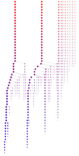
\includegraphics[width=5cm] {fel_tree}}
  \caption{\label{fig:fel_tree}
    Free energy landscape tree of Aib9 for $r=0.3$ and 500 frames minimal
    population per node.}
\end{figure}


\subsection{The resulting microstate trajectory}
To separate the tree at its 'leaf-branches', i.e., to assign all frames in the
trajectory to a distinct microstate, run
\begin{lstlisting}
  clustering density -f coords
                       -i network_end_node_traj.dat
                       -r 0.3
                       -D fe
                       -B nn
                       -o microstates
                       -n 12
                       -v
\end{lstlisting}

\begin{itemize}
  \item -i: By defining the clustered trajectory of basin centers, we seed the
            clustering process with a limited number of microstates.
            The \emph{clustering} program will use this information to assign
            all unassigned frames to one of these microstates.
            This is done by 'filling' the basins, i.e. starting at the
            unassigned frame of lowest free energy, it will identify the
            closest microstate and add the given frame to its population.
            With the updated clustering trajectory, this process is repeated
            until no frame is left unassigned.
  \item -o: The final microstate trajectory is written to the file specified
            with this option.
\end{itemize}

The end result of the geometric, density-based clustering is the 'microstates'
file, which holds a single column with microstate id / frame, where the row
number equals the according frame number. Due to the remapping during the
network generation (section \ref{sec:network_generation}) the resulting ids
may have large values and are generally not in consecutive order.
The advantage is, that the microstate ids are, however, unique and a
comparison / search in the remapped cluster files allows the identification of
the according basin center.


\begin{mdframed}[innertopmargin=20pt]
  Again, since we can reuse free energy and neighborhood information, above
  command is not compute intensive and finishes in short time.
\end{mdframed}



\section{Dynamical clustering with the Most-Probable-Path (MPP) method}
To get a dynamical description of the state space, use the MPP method to
cluster the geometric microstates by their respective transition probabilities.
This way, we identify the dynamically more stable from the less stable states.
The most important parameter for MPP is the lagtime, which is -- for the
\emph{clustering} program -- always given in numbers of frames.
The lagtime in units of time is trivially given by its value in numbers of
frames multiplied by the time step of the underlying simulation.

The lagtime is the amount of time (or number of frames) that is skipped when
calculating transition probabilities from one state to another.
In effect, timescales below the given lagtime are discarded and the dynamical
clustering will only be able to describe processes of length higher then then
given lagtime. It acts as a control parameter to blend out (uninteresting)
processes on too short timescales and focus on processes of essential motion,
which typically happen at longer timescales as the simulation stepping.

Additionally, at a high enough lagtime the system will be approximately
markovian, resulting in a discrete set of states well described by markovian
dynamics.

To run MPP, use the command
\begin{lstlisting}
  clustering mpp -i microstates
                   -D fe
                   -B nn
                   -l 50
                   -v
\end{lstlisting}

\begin{itemize}
  \item -i: The cluster trajectory of microstates as input. Here, we use the
            'microstates' file from the previous step.
  \item -l: The lagtime as number of frames.
\end{itemize}

The MPP run generates lots of new files, per default called 'mpp\_pop\_*' and
'mpp\_traj\_*'. The star stands for the metastability ($Q_\text{min}$-value)
of the run. The *pop*-files hold the population information of the clusters
for the given metastibility, while the *traj*-files are the resulting cluster
trajectories.

The metastability value controls, how stable a state has to be to remain as
single state. All states with a stability less then the given
$Q_\text{min}$-value will be lumped according to their most probable state-path.

Let's assume from now on that the clustering resolution of choice is given at
a metastability of 0.98. Thus, the clustered trajectory is in the file
mpp\_traj\_0.98.


\section{Variable dynamic coring for state boundary corrections}
Transitions between states usually do not occur in a direct and discrete manner.
Rather, the system goes into a 'transition zone', where frames are alternating
fast between two states before staying in the new state.
These alternations severely change the dynamical description of the system and
produce artificially short life times.
You can use variable dynamic coring to correct for these boundary artifacts.
Here, 'dynamic' means that we refer to the core of a state, if the system stays
inside for a given amount of time (the coring window). Thus, we check dynamic
properties instead of geometric ones. The 'variable' part means that we define
the coring windows variably per state instead of defining one global coring
window for all states.

To identify the optimal coring window, run the coring-algorithm for several
different windows and plot the waiting time distributions per state and window.
The optimal window size is the one that best matches an exponential decay.
The reasoning follows the same logic as before with the cluster radii.

To produce waiting time distribution for different coring windows, write a
{\ttfamily win} file with the content
\begin{lstlisting}[language=bash,basicstyle=\ttfamily]
  * WINDOW_SIZE
\end{lstlisting}
where {\ttfamily WINDOW\_SIZE} is the window size given as number of frames.
The star means, that we treat all states with the same window size.

Then run the command
\begin{lstlisting}
  clustering coring -s mpp_traj_0.98
                      -w win
                      -d wtd
                      -v
\end{lstlisting}

This produces several files of the format {\ttfamily wtd\_STATE\_WINDOW}.
Repeat this process several times for different choices of window size in the
{\ttfamily win} file.

When you have selected proper windows sizes for all states, rewrite your
{\ttfamily win} file to reflect these. For the three different states 1, 2
\& 3, e.g. you could write
\begin{lstlisting}[basicstyle=\ttfamily]
  1 100
  2 200
  3 75
\end{lstlisting}
for window sizes of 100 frames for state 1, 200 frames for state 2 and 75
frames for state 3.

Finally, to produce the cored cluster trajectory, run
\begin{lstlisting}
  clustering coring -s mpp_traj_0.98
                      -w win
                      -o clustered_traj
                      -v
\end{lstlisting}

\bibliographystyle{plain}
\bibliography{ref}

\end{document}
